\documentclass[12pt,letterpaper]{article}
\usepackage[utf8]{inputenc}
\usepackage[spanish]{babel}
\usepackage{graphicx}
\usepackage[left=2cm,right=2cm,top=2cm,bottom=2cm]{geometry}
\usepackage{graphicx} % figuras
% \usepackage{subfigure} % subfiguras
\usepackage{float} % para usar [H]
\usepackage{amsmath}
%\usepackage{txfonts}
\usepackage{stackrel} 
\usepackage{multirow}
\usepackage{enumerate} % enumerados
\renewcommand{\labelitemi}{$-$}
\renewcommand{\labelitemii}{$\cdot$}
% \author{}
% \title{Caratula}
\begin{document}

% Fancy Header and Footer
% \usepackage{fancyhdr}
% \pagestyle{fancy}
% \cfoot{}
% \rfoot{\thepage}
%

% \usepackage[hidelinks]{hyperref} % CREA HYPERVINCULOS EN INDICE

% \author{}
\title{Caratula}

\begin{titlepage}
\begin{center}
\large{UNIVERSIDAD PRIVADA DE TACNA}\\
\vspace*{-0.025in}
\begin{figure}[htb]
\begin{center}

\includegraphics[width=4cm]{./Imagenes/logo}
\end{center}
\end{figure}
\vspace*{0.15in}
INGENIERIA DE SISTEMAS  \\

\vspace*{0.5in}
\begin{large}
TEMA:\\
\end{large}

\vspace*{0.1in}
\begin{Large}
\textbf{Comparativa Business Intelligence vs Business Analytics} \\
\end{Large}

\vspace*{0.3in}
\begin{Large}
\textbf{CURSO:} \\
\end{Large}

\vspace*{0.1in}
\begin{large}
INTELIGENCIA DE NEGOCIOS\\
\end{large}

\vspace*{0.3in}
\begin{Large}
\textbf{DOCENTE(ING):} \\
\end{Large}

\vspace*{0.1in}
\begin{large}
 Patrick Jose Cuadros Quiroga\\
\end{large}

\vspace*{0.2in}
\vspace*{0.1in}
\begin{large}
Integrantes: \\
\begin{flushleft}

Samuel Ray NÚÑEZ MAMANI         	\hfill	(2016054462) \\
Jorge Luis MAMANI MAQUERA    	           \hfill	(2016055236) \\
Katerin Almendra MERINO QUISPE	\hfill	(2018060918) \\
Jhony José MAMANI LIMACHE		\hfill	(2013046566) \\

\end{flushleft}
\end{large}
\end{center}

\end{titlepage}


\tableofcontents % INDICE
\thispagestyle{empty} % INDICE SIN NUMERO
\newpage
\setcounter{page}{1} % REINICIAR CONTADOR DE PAGINAS DESPUES DEL INDICE

\section{RESUMEN Y ABSTRACT} 
\begin{flushleft}

\textbf{Resumen}\\
En los ultimos años, las organizaciones han recurrido cada vez mas a soluciones de software
avanzadas para administrar las cargas de trabajo, mantener la rentabilidad y asegurar la
competitividad dentro de sus respectivas industrias. Si bien hay varias opciones disponibles,
las herramientas de inteligencia de negocios (BI) y las herramientas de analisis de negocios
(BA) son posiblemente las soluciones de administracion de datos mas implementadas. Los
analistas de negocios y los compradores de software a menudo preguntan cuales son las diferencias
clave entre la inteligencia de negocios y los analisis de negocios.
\textbf{}\\
\textbf{}\\

\textbf{Abstract}\\
In recent years, organizations have increasingly turned to advanced software
solutions to manage workloads, maintain protability and ensure competitiveness
within their respective industries. While there are several options available, business
intelligence tools (BI) and business analytics tools (BA) are arguably the most
widely implemented data management solutions. Business analysts and software
buyers alike often ask what are the key diferences between business intelligence vs business analytics.












\end{flushleft}
\section{INTRODUCCION} 
\textbf{}\\
\begin{flushleft}
\textbf {¿Qué es Microsoft Visual Studio?}\\

\textbf{}\\
\textbf{}\\
\textbf {¿Qué es Microsoft SQL Server?}\\
Microsoft SQL Server es un sistema de gestión de base de datos relacional, desarrollado por la empresa Microsoft.\textbf{}\\


\textbf{}\\
\textbf{}\\
\textbf {¿Qué es un Diagrama de Caso de Uso?}\\

\textbf{}\\

\textbf{}\\


\textbf{}\\
\textbf{}\\
\textbf {¿Qué es un Diagrama de Clases?}\\

\textbf{}\\
\textbf{}\\
\textbf {¿Qué es un Diagrama de Entidad – Relación?}\\

\textbf{}\\
\textbf{}\\
\textbf {¿Qué es ORM?}
\textbf{}\\






 

\end{flushleft}
\section{MARCO TEÓRICO} 
\begin{flushleft}
\textbf {1.1 INTELIGENCIA DE NEGOCIOS}\\
\textbf{}\\
La inteligencia de negocios se define como la habilidad corporativa para tomar decisiones. Esto se logra mediante el uso de metodologías, aplicaciones y tecnologías que permiten reunir, depurar, transformar datos, y aplicar en ellos técnicas analíticas de extracción de conocimiento (Parr 2000), los datos pueden ser estructurados para que indiquen las características de un área de interés (Stackowiak et al. 2007), generando el conocimiento sobre los problemas y oportunidades del negocio para que pueden ser corregidos y aprovechados respectivamente. (Ballard et al. 2006) 

Implementar herramientas de BI dentro de la organización permite soportar las decisiones que se toman; al nivel interno ayuda en la gestión del personal (Sharma et al. 2009) y del lado externo produce ventajas sobre sus competidores (Maureen 2009). Existen ocasiones en las cuales no se pueden lograr todos los beneficios que tiene BI; debido al proceso que lleva consigo implementar un proyecto de estas características, se puede cometer errores en la definición del planteamiento de las necesidades de conocimiento de la empresa; el no determinar la magnitud de los problemas de información a solucionar generalmente repercute en el fracaso del proyecto.\textbf{}\\
\textbf{}\\
En la actualidad se está planteando un concepto nuevo llamado Agile BI Governance, el cual propone, arquitecturas, métodos y herramientas necesarios para implantar una infraestructura para BI. Esta definición, combina conceptos de IT Governance, Manifiesto Ágil y Data Governance, para lograr un alcance que contemple las diferentes unidades de negocio, y soporte el proceso estratégico de obtención de valor del Business Intelligence en la empresa. Permite conocer cómo controlar un sistema de estas características, qué políticas debo aplicar, qué métodos de control tengo que poner en marcha y cómo debo gobernar los sistemas de BI. (Fernández 2008) \textbf{}\\
\textbf{}\\
Agile BI Governance establece 4 valores básicos, pero dependiendo de cada organización puede incluir los que vayan en relación con su propia estrategia. \textbf{}\\
\textbf{}\\
\item • \textbf{Adaptabilidad Continúa.} La incertidumbre y el cambio continuo son el estado natural de los sistemas de toma de decisiones, pero parece ser que muchas organizaciones aún no son conscientes de ellos. En este tipo de proyectos siempre se está cambiando el punto de vista analítico. \textbf{}\\
\item • \textbf{Trabajo Conjunto.}  El usuario operativo del software ha de ser parte activa dentro de los grupos de IT que desarrollan los sistemas de BI.\textbf{}\\
\item • \textbf{Jerarquías Flexibles.} Los grupos de trabajo dentro del Agile BI Governance deberán estar estructurados con jerarquías flexibles que fomenten el intercambio de información. \textbf{}\\
\item • \textbf{Personas Antes que Procesos.}  Priorizar la entrega de la información a las personas que controlan los procesos y no tanto en definir los procesos que han de controlar las personas. (Fernández 2008)

\textbf{}\\
\textbf{}\\
\textbf{}\\
\textbf{}\\
\textbf{}\\
\textbf{}\\
\textbf {1.2 DATA WAREHOUSE}\\
\textbf{}\\
Es el proceso de extraer datos de distintas aplicaciones (internas y externas), para que una vez depurados y especialmente estructurados sean almacenados en un depósito de datos consolidado para el análisis del negocio. Requiere una combinación de metodologías, técnicas, hardware y los componentes de software que proporcionan en conjunto la infraestructura para soportar el proceso de información (Stackowiak et al. 2007). La estructura que se defina debe reflejar las necesidades y características del negocio, sus departamentos, equipos de trabajo y directivos1 , esto permitirá responder a interrogantes generados al tratar de tomar las decisiones (Witten 2000) y con el tiempo se va convirtiendo en la memoria corporativa (Wang 2009); describiendo el pasado y el presente de la empresa. Data Warehouse desglosa, resume, ordena y compara, pero no descubre, ni predice. (Flores 2004) 

\textbf{}\\
Para la construcción de un Data Warehouse se establecen tres etapas; la primera está dedicada a examinar el esquema Entidad Relación de la base de datos operacional, generando los esquemas multidimensionales candidatos. 

\textbf{}\\
La segunda etapa, consiste en recoger los requisitos de usuario por medio de entrevistas, para obtener información acerca de las necesidades de análisis de estos, y la tercera etapa, contrasta la información obtenida en la segunda etapa, con los esquemas multidimensional candidatos formados en la primera etapa generando así, una solución que refleja los requisitos de usuario (Zenaido 2008). 

\textbf{}\\
Por otra parte implementar una solución de este tipo, ocasiona un costo que no todas las organizaciones están dispuestas a pagar (debido a sus capacidades de inversión), es por eso que los promotores del proyecto dentro de la empresa deben persuadir a los directivos y compañeros de trabajo, una buena alternativa de hacerlo es mediante el uso de técnicas administrativas, que permitan conocer a los directivos como se puede establecer el retorno de la inversión del proyecto equiparando inversión contra beneficios. (Arturo 2001)

\textbf{}\\
Al ser un depósito de datos consolidado para el análisis del negocio necesita tomar datos de distintas fuentes, Internas y Externas (Stackowiak et al. 2007), y como las características de las empresas son diferentes la cantidad de registros almacenados en algunas de ellas puede llegar a ser de proporciones exponenciales; es por esta razón que se necesita de procesos que optimicen los tiempos de extracción, transformación y transferencia de los datos del sistemas de información a la fuente de datos esto se logra implementando técnicas incrementales que mediante el uso de Snapshots y Triggers, se encarguen de sacar, transformar y transferir los registros que existen en el sistema de información a la fuente de datos. (Flores 2003)

\textbf{}\\

El uso de Data Warehouse es tan amplio que llega a diferentes tipos de organizaciones y distintos temas de interés, puede ser implementado con conceptos Administrativos, en la administración; ayuda en la identificación de elementos de cambio que definan una nueva manera de hacer negocios, en donde la competencia debe estar orientada a trabajar no sólo de forma aislada, sino en colaboración con los diversos grupos de interés o actores de la industria, buscando referencias diferenciadoras para alcanzar el éxito (Romero 2002), en empresas petroquímicas; incrementa la exactitud y precisión en la toma de decisiones con un 93.9\% en la rentabilidad (Silva 2009), en la Web; optimiza búsqueda Web de metadatos con características semi-inteligentes y también suministra el soporte necesario para crear comunidades de colaboración científica (Luna et al. 2008) (Ameur et al. 2006), en transformadores de potencia; almacenando, la monitorización del estado del flujo de energía (Mariño et al. 2004).
\textbf{}\\
\textbf{}\\
\textbf{1.3 OLAP}\\
El procesamiento analítico en línea permite obtener acceso a datos organizados y agregados de orígenes de datos empresariales2 , organiza subconjuntos de datos con una estructura multidimensional de manera que represente un significado especial o responda a una pregunta en particular 3 4 . (Roussel 2006) Estas herramientas soportan el análisis interactivo de la información de resumen, soportando muchas tareas de agrupación de datos que no pueden realizarse empleando las facilidades básicas de agregación y agrupamiento (Silberschatz et al. 2006)\textbf{}\\
\textbf{}\\
\textbf{1.3.1 TIPOS DE SISTEMAS OLAP}\\
Tradicionalmente, este sistema se clasifica según las siguientes categorías: 
\textbf{}\\
\item • \textbf{ROLAP.} Implementación que almacena los datos en un motor relacional. Típicamente, los datos son detallados, evitando las agregaciones y las tablas se encuentran normalizadas. \textbf{}\\

\item • \textbf{MOLAP.} Esta implementación almacena los datos en una base de datos multidimensional. Para optimizar los tiempos de respuesta, el resumen de la información es usualmente calculado por adelantado. \textbf{}\\

\item • \textbf{ HOLAP(Hybrid OLAP).} Almacena algunos datos en un motor relacional y otros en una base de datos multidimensional5 .
\textbf{}\\
\textbf{}\\
Al igual que Data Warehouse, OLAP también es aplicable a un amplio rango de temas diferentes, uno de ellos es en Bases de Datos espaciales proporcionando características necesarias para los sistemas de tipo geográfico; como hechos, dimensiones, miembros, niveles, jerarquías, operaciones de navegación, operaciones de consolidación y comportamiento del clima (Abril 2007) (Bernier et al. 2009). También se utiliza el almacenamiento MOLAP y ROLAP, para generar índices que mejoran los tiempos de accesos a las consultas de manera que los tiempos de entrega de la información demore el menor tiempo posible (Tamayo 2006). Otra de las aplicaciones es en la educación al ser aplicado en ambientes de aprendizaje proporcionando las dimensiones y los indicadores necesarios para hacer la definición de un modelo de evaluación académica (Cockbaine 2004).\textbf{}\\
\textbf{}\\
 \textbf{1.4 CUADRO DE MANDO INTEGRAL}\\
\textbf{}\\
El cuadro de mando integral (Balanced Scorecard) es una herramienta que permite alinear los objetivos de las diferentes áreas o unidades con la estrategia de la empresa y seguir su evolución6. El uso que se le puede dar a un Cuadro de Mando Integral es tan diverso que se puede contemplar autoevaluaciones del personal (Martínez 2008), hasta la definición de conceptos netamente organizacionales como son; la misión, la política de calidad; plan de comunicación, imagen corporativa, acciones de formación, catálogo de servicios; la confección de una cartera de clientes y la realización de acciones para conocer mejor sus opiniones y preferencias, así como para personalizar la presentación de la oferta de servicios para los clientes más importantes (Villalbía et al. 2005) (Matilla 2007). En fin, la ejecución de un cuadro de mando es tan amplia y generosa que puede llegar a cambiar la forma en que se presta un servicio en entidades públicas (Peters et al. 2007) (Weir et al. 2009).\textbf{}\\
\textbf{}\\
\textbf{1.5 DATA MINING }\\
\textbf{}\\
Es el proceso de Seleccionar, Explorar, Modificar, Modelizar7 y valorar grandes cantidades de datos con el objetivo de descubrir conocimiento (Pérez 2006). El proceso debe ser automático o semi-automático. Los modelos hallados deben ser significativos demostrando cierto patrón o regla de comportamiento8 . Las aplicaciones más utilizadas son las que necesitan algún tipo de predicción. Por ejemplo, cuando una persona solicita una tarjeta de crédito, la compañía emisora quiere predecir si la persona, clasifica con el perfil identificado de usuarios morosos (Silberschatz et al. 2006). \textbf{}\\
\textbf{}\\
La minería de datos, permite la gestión en tiempo real de manera eficaz, es una herramienta aplicable a cualquier tipo de empresa. Una amplia gama de compañías puede tener aplicaciones exitosas con ella (Angeles et al. 2010). \textbf{}\\
\textbf{}\\
Beneficios asociados a la minería de datos (López 2004): Incremento de los resultados como consecuencia del aumento de la cuota de mercado; Fidelización de la clientela dada una mejor respuesta a sus requerimientos; Mejora del rendimiento; Reducción del factor riesgo; Optimización de las estrategias y toma de decisiones y Optimización de la gestión, maximizando rentabilidades. \textbf{}\\
\textbf{}\\
La aplicación de la Minería de Datos, además de permitir el descubrimiento del conocimiento en general, también se utiliza Biología soporta las investigaciones en la rama biológica, como herramienta insustituible para enfrentar la avalancha de datos que producen esta clase de proyectos (Febles 2002), en la Web Semántica; convierte la información en conocimiento que está distribuida en la web, proporcionando a las computadoras una mayor capacidad para gestionar y recuperar dichos datos (Rodríguez 2006), en las Redes de computadores; mediante la recolección de información acerca de los factores que impactan sobre la infraestructura de seguridad para descubrir la información relevante que ayude a tomar decisiones para corregir y/o mejorar las infraestructura de seguridad (Rojas 2005), en la Educación; haciendo seguimiento en los procesos de auto aprendizaje (Radenkovic et al. 2009).


\textbf{}\\
\textbf{}\\
\textbf{}\\
\textbf{}\\
\textbf{}\\
\textbf{}\\
\textbf{}\\
\textbf{}\\
\textbf{}\\
\textbf{}\\
\textbf{}\\
\textbf{}\\
\textbf{}\\
\textbf{}\\
\textbf{}\\
\textbf{}\\
\textbf{2.1 ANALISIS DE NEGOCIOS}\\
\textbf{}\\
El análisis de negocio(Business Analytics, BA) es el conjunto de métodos y técnicas utilizadas para trabajar como enlace entre los stackeholders, con el fin de comprender la estructura, políticas y operaciones de una organización y recomendar soluciones que permitan a la organización alcanzar sus objetivos (IIBA: International Institute of Business Analysis).\\
\textbf{}\\
El análisis de negocios implica la comprensión de cómo funcionan las organizaciones para llevar a cabo sus propósitos, y la definición de las capacidades que una organización requiere para proporcionar productos y servicios a los grupos de interés externos. Incluye la definición de los objetivos de la organización, cómo esos objetivos se conectan a objetivos específicos, que determinan las líneas de acción que una organización tiene que realizar para alcanzar esas metas y objetivos, y definir cómo las distintas unidades de organización y las partes interesadas dentro y fuera de esa organización interactúa.
\begin{center}
		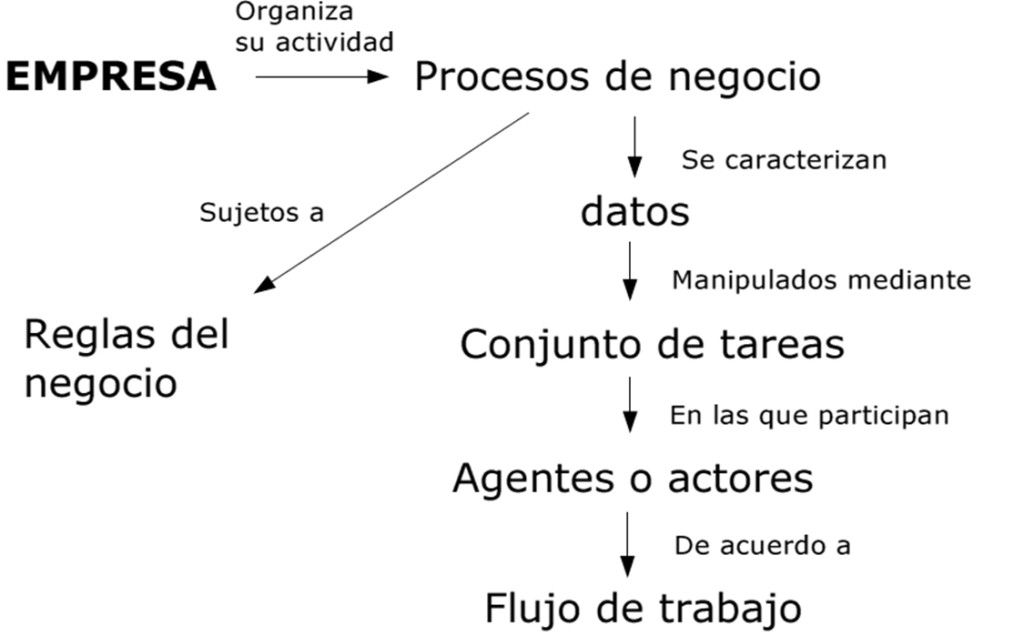
\includegraphics[width=15cm]{./Imagenes/anegocios}
		\end{center}

\textbf{}\\
\textbf{}\\

\textbf{2.2 Aplicaciones de Analisis de Negocios}\\
Las herramientas de inteligencia de negocio son aplicaciones digitales diseñadas para colaborar con el Business Intelligence durante el análisis y la presentación de datos.\\
La Inteligencia de Negocios o Business Intelligence (BI) permite a las compañías contar con la información adecuada para una mejor toma de decisiones.  Las compañías que implementan el BI logran sacar mayor provecho de las situaciones de crisis gracias a la posibilidad de contar con un análisis de mercado más acertado debido a que los datos pesados son transformados en importantes estrategias corporativas.
Actualmente, las herramientas de BI disponibles en el mercado son incontables, pero estas 20 no pueden pasar desapercibidas:
\textbf{}\\
\textbf{}\\
\textbf{}\\

\textbf{2.2.1. Microsoft Dynamics NAV: }\\
Especial para pequeñas y medianas empresas que buscan mejorar su competitividad.
	\begin{center}
	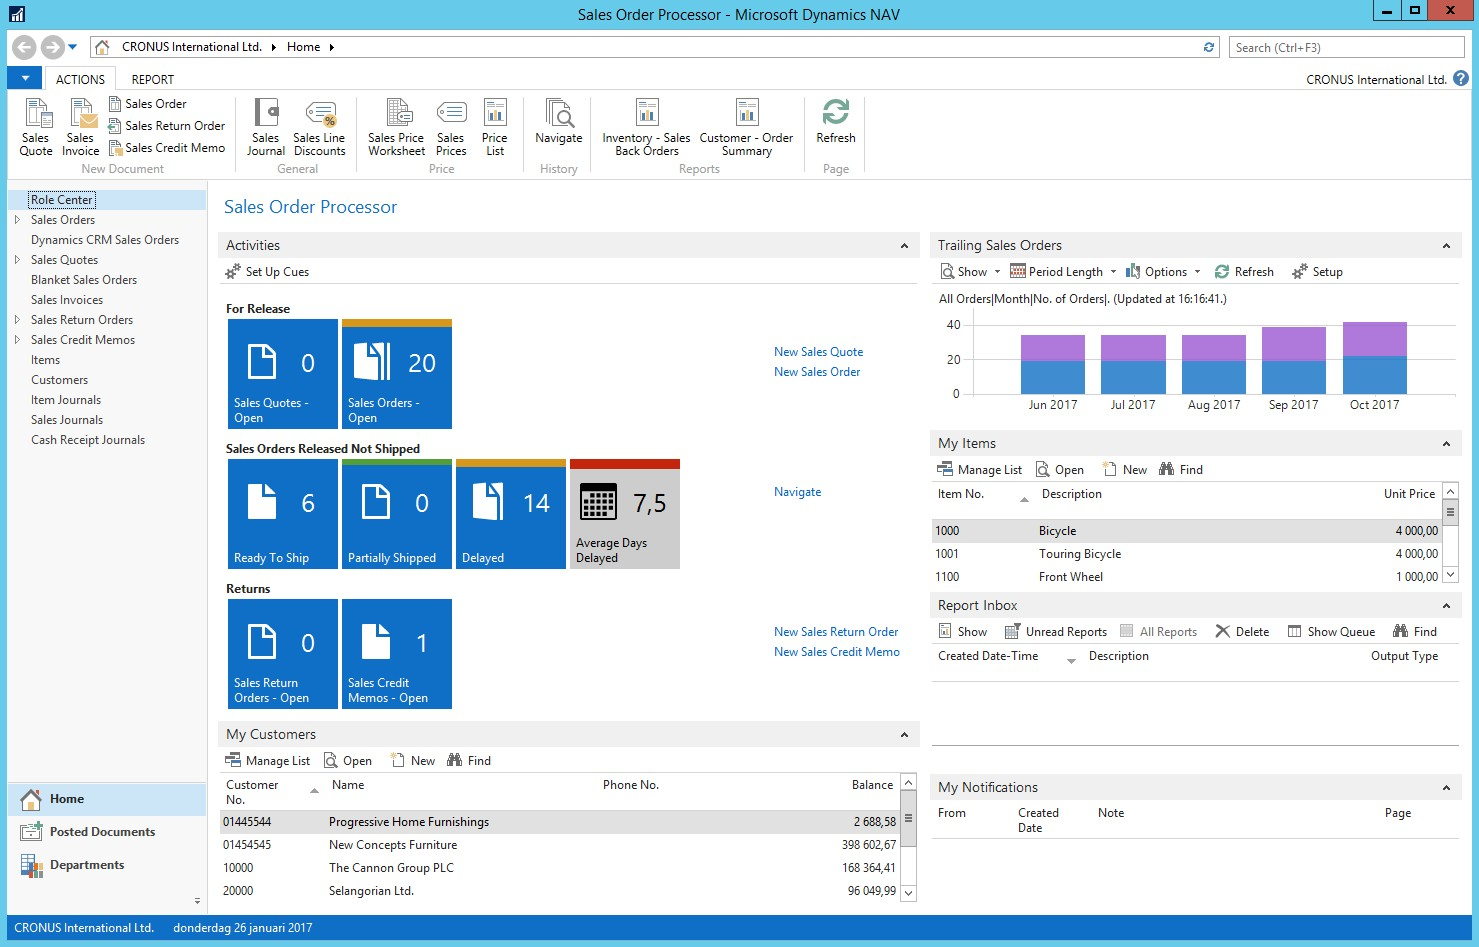
\includegraphics[width=15cm]{./Imagenes/BIimagen1}
	\end{center}
	
\textbf{}\\
\textbf{2.2.2. Microsoft Dynamics CRM: }\\
Efectiva para la administración de clientes.
	\begin{center}
	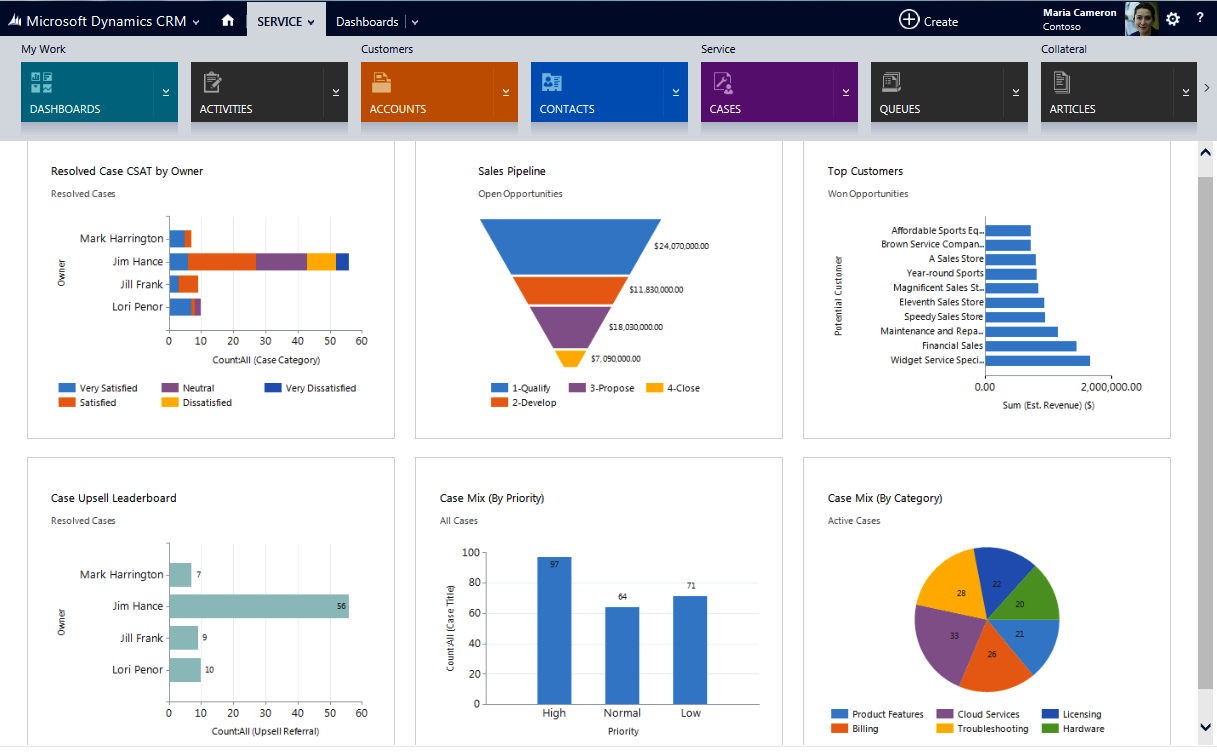
\includegraphics[width=12cm]{./Imagenes/BIimagen2}
	\end{center}
	\textbf{}\\
\textbf{}\\
\textbf{}\\
\textbf{}\\

\textbf{}\\
\textbf{}\\
\textbf{}\\
\textbf{2.2.3. Oracle Business Intelligence: }\\
Una de las más completas en el mercado ya que cuenta con paneles interactivos, análisis predictivos en tiempo real, entre otros.
	\begin{center}
	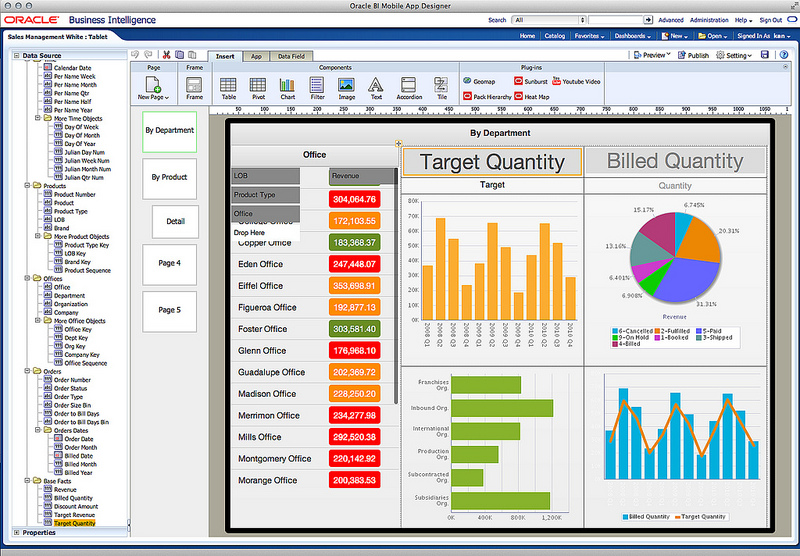
\includegraphics[width=12cm]{./Imagenes/BIimagen3}
	\end{center}
	\textbf{}\\

\textbf{2.2.4. Ultimus: }\\
Un entorno integrado que permite compartir información entre aplicaciones.
	\begin{center}
	
\includegraphics[width=12cm]{./Imagenes/BIimagen4}
	\end{center}
	
\textbf{}\\
\textbf{}\\
\textbf{}\\
\textbf{}\\
\textbf{}\\
\textbf{2.2.5. Office SharePoint Server: }\\
Facilita el acceso a la información en cualquier momento y lugar.
	\begin{center}
	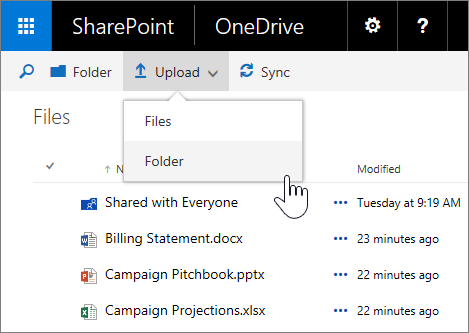
\includegraphics[width=12cm]{./Imagenes/BIimagen5}
	\end{center}
	\textbf{}\\

\textbf{2.2.6. QlikView: }\\
Mantiene las bases de datos al alcance de una manera sin precedentes.
	\begin{center}
	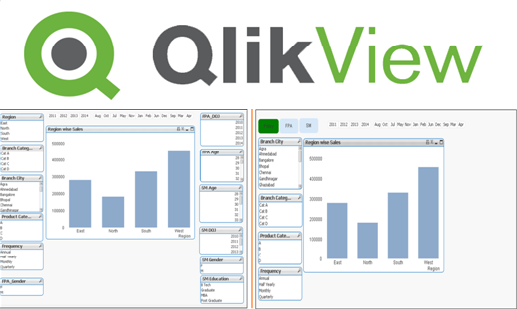
\includegraphics[width=15cm]{./Imagenes/BIimagen6}
	\end{center}
\textbf{}\\
	\textbf{}\\
\textbf{}\\
\textbf{}\\
\textbf{}\\
\textbf{}\\
\textbf{}\\
\textbf{2.2.7. Microsoft Performance Point Server: }\\
Permite supervisar, alinear y hacer un plan de negocio.
	\begin{center}
	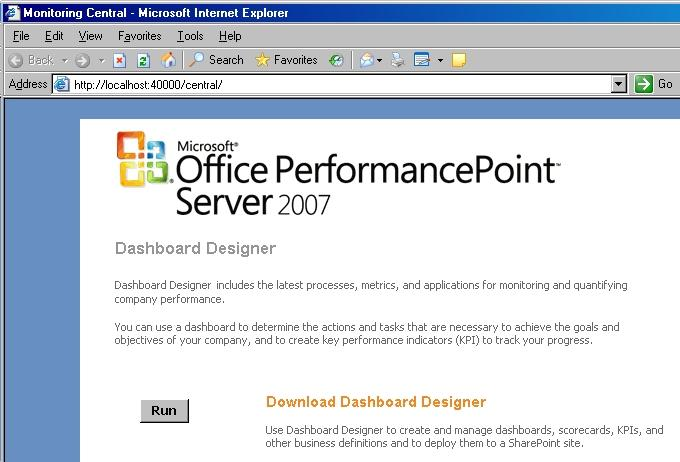
\includegraphics[width=15cm]{./Imagenes/BIimagen7}
	\end{center}
\textbf{}\\
	
\textbf{2.2.8. Microsoft SQL Server: }\\
Adecuada para realizar un análisis panorámico de la empresa y tomar las mejores decisiones.
	\begin{center}
	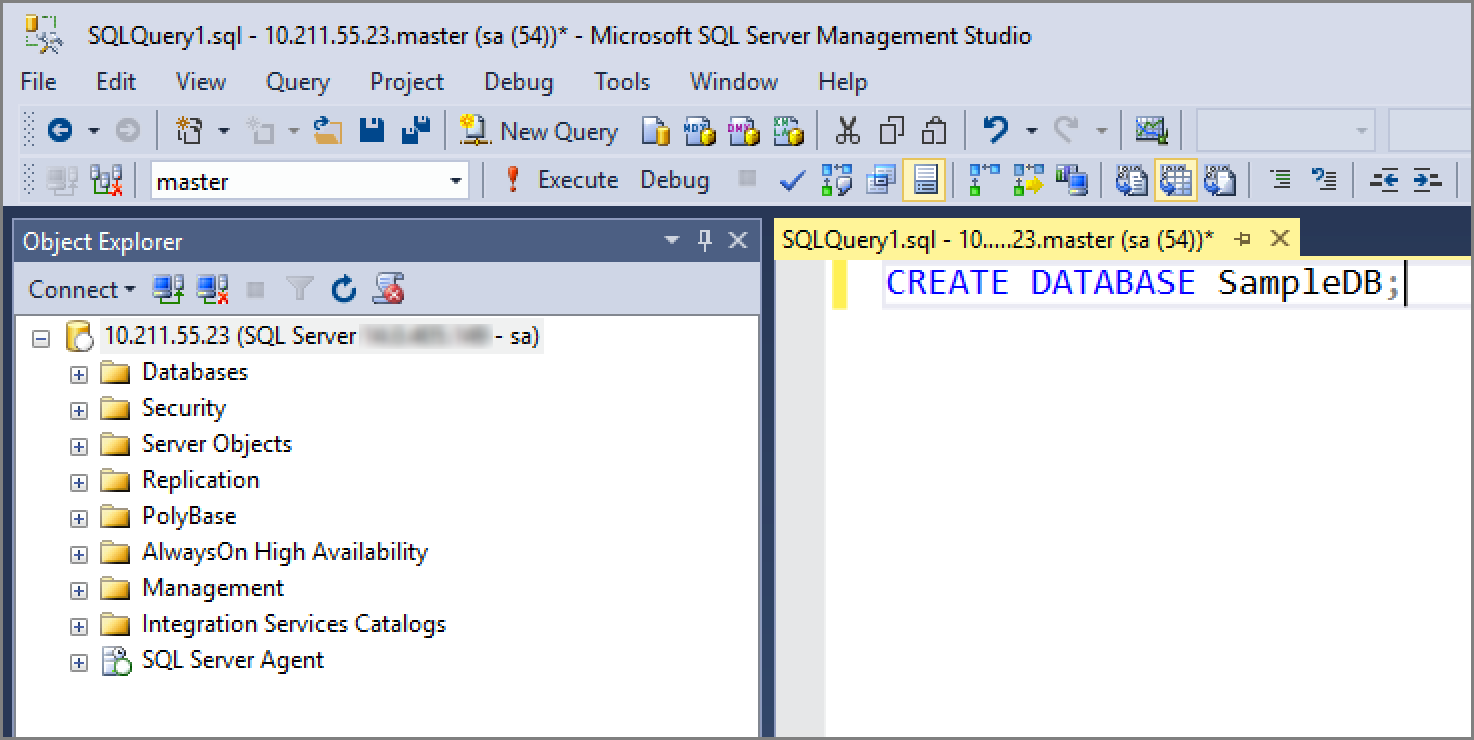
\includegraphics[width=10cm]{./Imagenes/BIimagen8}
	\end{center}
\textbf{}\\
	\textbf{}\\
\textbf{}\\
\textbf{}\\
\textbf{}\\
\textbf{}\\
	\textbf{}\\
\textbf{}\\
\textbf{}\\
\textbf{}\\
\textbf{}\\
\textbf{2.2.9. JetReports: }\\
Especial para crear informes ERP.
	\begin{center}
	
\includegraphics[width=10cm]{./Imagenes/BIimagen9}
	\end{center}
\textbf{}\\
	
\textbf{2.2.10. Eclipse BIRT Project: }\\
Genera informes para aplicaciones web de código abierto.
	\begin{center}
	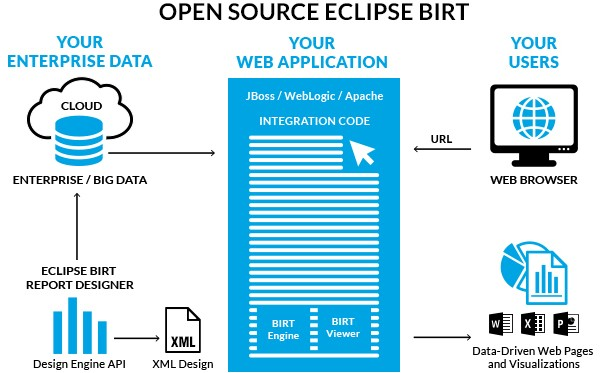
\includegraphics[width=10cm]{./Imagenes/BIimagen10}
	\end{center}
\textbf{}\\
	
\textbf{2.2.11. JasperReports: }\\ 
Permite crear informes de rápida impresión.
	\begin{center}
	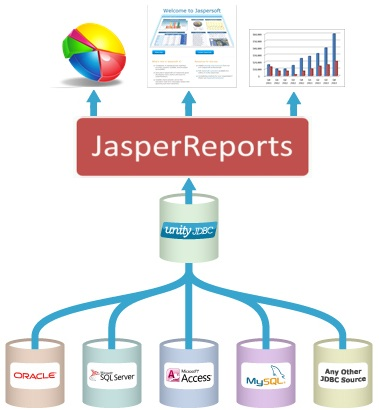
\includegraphics[width=7cm]{./Imagenes/BIimagen11}
	\end{center}
\textbf{}\\
	
\textbf{2.2.12. LogiReport: }\\
Aplicación gratuita basada en web de LogiXML
	\begin{center}
	
\includegraphics[width=12cm]{./Imagenes/BIimagen12}
	\end{center}
\textbf{}\\
	
\textbf{2.2.13. OpenI: }\\
Aplicación web orientada al reporting OLAP.
	\begin{center}
	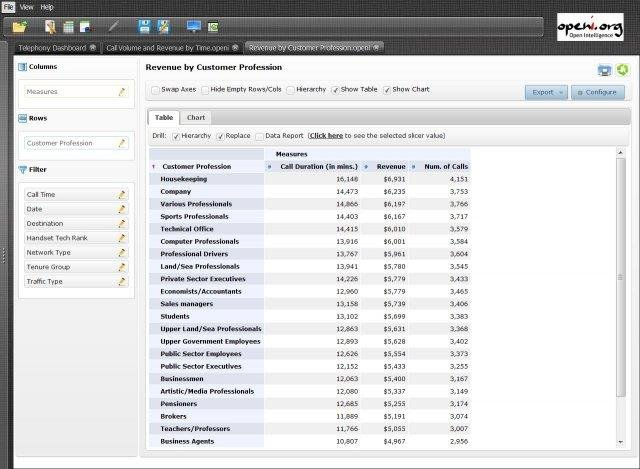
\includegraphics[width=12cm]{./Imagenes/BIimagen13}
	\end{center}
\textbf{}\\
\textbf{}\\
\textbf{}\\
\textbf{}\\
\textbf{}\\
	\textbf{}\\
\textbf{}\\
\textbf{}\\
\textbf{}\\	
\textbf{}\\
\textbf{}\\	
\textbf{}\\
\textbf{}\\
\textbf{2.2.14. SPSS: }\\
Programa estadístico especialmente empleado en ciencias sociales e investigaciones de mercado.
	\begin{center}
	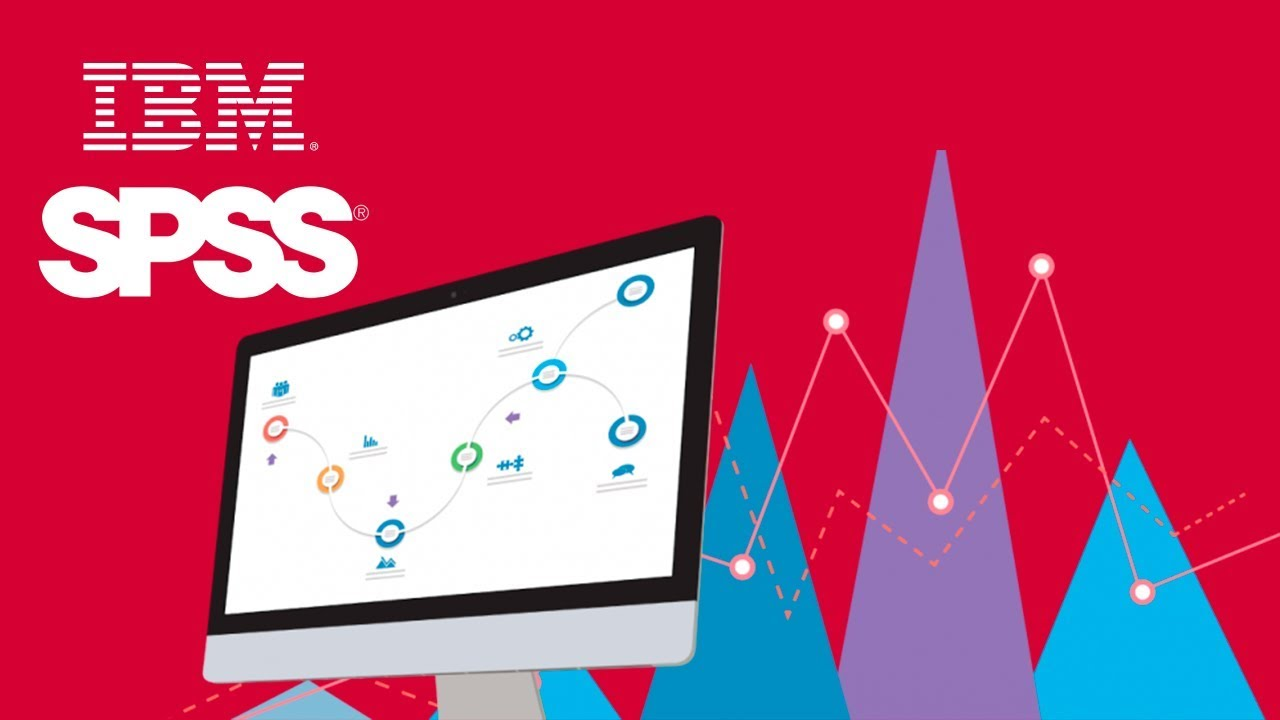
\includegraphics[width=13cm]{./Imagenes/BIimagen14}
	\end{center}
\textbf{}\\
	
\textbf{2.2.15. Pentaho: }\\ 
Incluye herramientas para generar informes, minería de datos, ETL, entre otros.
	\begin{center}
	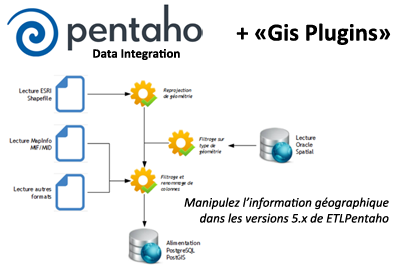
\includegraphics[width=10cm]{./Imagenes/BIimagen15}
	\end{center}
\textbf{}\\
	
\textbf{2.2.16. RapidMiner: }\\
Permite analizar datos a través de un entorno gráfico.
	\begin{center}
	
\includegraphics[width=10cm]{./Imagenes/BIimagen16}
	\end{center}

\textbf{}\\
\textbf{}\\
\textbf{}\\
\textbf{2.2.17. Crystal Reports: }\\
Genera informes desde bases de datos múltiples.
	\begin{center}
	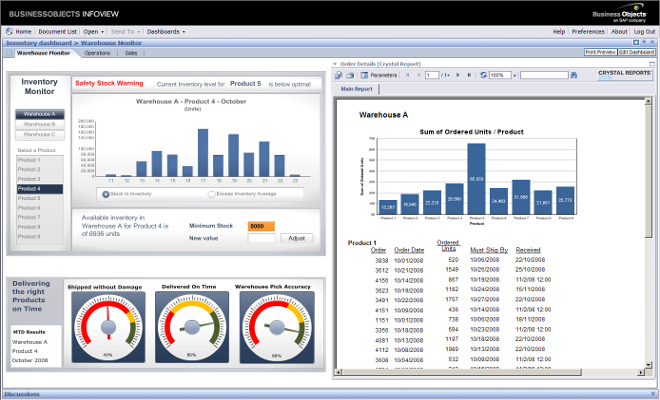
\includegraphics[width=10cm]{./Imagenes/BIimagen17}
	\end{center}

\textbf{}\\
\textbf{2.2.18. ApeSoft: }\\
Ofrece una interface sencilla similar a Microsoft Excel.
	\begin{center}
	
\includegraphics[width=9cm]{./Imagenes/BIimagen18}
	\end{center}
\textbf{}\\
	
\textbf{2.2.19. SAS Institute: }\\ 
Facilita la gestión de riesgo financiero, desarrollo de modelos de minería de datos, etc.
	\begin{center}
	
\includegraphics[width=7cm]{./Imagenes/BIimagen19}
	\end{center}
\textbf{}\\
	\textbf{}\\
\textbf{}\\
\textbf{}\\
\textbf{}\\
\textbf{2.2.20. NiMbox: }\\
Organiza los datos de la empresa en interactivas aplicaciones.
	\begin{center}
	
\includegraphics[width=8cm]{./Imagenes/BIimagen20}
	\end{center}







\textbf{}\\
\end{flushleft}
\section{ANALISIS} 
\begin{flushleft}
\textbf {3.1 ANALISIS (Casos de Uso)}\\

\textbf{}\\

\textbf{}\\
\textbf{}\\
\textbf{}\\
\textbf{}\\
\textbf{}\\
\textbf{}\\
\textbf{}\\
\textbf{}\\
\textbf{}\\
\textbf{}\\
\textbf{}\\
\textbf{}\\
\textbf{}\\
\textbf{}\\
\textbf{}\\
\textbf{}\\
\textbf{}\\
\textbf{}\\
\textbf {3.2 DISEÑO (Diagrama de Clases, Modelo Entidad Relación)}\\
\textbf{}\\
\textbf {Diagrama de Clases}\\
\textbf{}\\
\textbf{}\\
\textbf{}\\
\textbf{}\\
\textbf{}\\
\textbf{}\\
\textbf{}\\

\textbf{}\\
\textbf{}\\
\textbf{}\\
\textbf{}\\
\textbf{}\\
\textbf{}\\
\textbf {3.3 PRUEBAS UNITARIAS}\\
\textbf{}\\

\end{flushleft}
\section{CONCLUSIONES} 
\begin{flushleft}
\textbf {3.1 ANALISIS (Casos de Uso)}\\

\textbf{}\\
\textbf{}\\
\textbf{}\\
\textbf{}\\
\textbf{}\\
\textbf{}\\
\textbf{}\\
\textbf{}\\
\textbf{}\\
\textbf{}\\
\textbf{}\\
\textbf{}\\
\textbf{}\\
\textbf{}\\
\textbf{}\\
\textbf{}\\
\textbf{}\\
\textbf{}\\
\textbf{}\\
\textbf {3.2 DISEÑO (Diagrama de Clases, Modelo Entidad Relación)}\\
\textbf{}\\
\textbf {Diagrama de Clases}\\
\textbf{}\\
\textbf{}\\
\end{flushleft}
\section{BIBLIOGRAFIA} 
\begin{flushleft}




\textbf {http://revistas.utp.edu.co/index.php/revistaciencia/article/view/1803/1209}\\

\textbf{https://www.sciencedirect.com/science/article/pii/S0186104215000807}\\

\textbf{http://www.spentamexico.org/v4-n2/4(2)\%2016-52.pdf}\\

\textbf{https://selecthub.com/business-intelligence/business-intelligence-vs-business-analytics}\\
\textbf{https://www.betterbuys.com/bi/business-intelligence-vs-business-analytics}\\
\textbf{https://aprendebi.wordpress.com/2016/11/30/bussiness-intelligence-vs-bussiness-analytics}\\
\textbf{http://scholarium.info/analisis-de-negocio-business-analysis-ba}\\
\textbf{https://blog.corponet.com.mx/que-es-la-inteligencia-de-negocios}\\











\textbf{}\\



\textbf{}\\

\end{flushleft}




\end{document}